\subsection{Excercise OrchestrationDiagramRentACar}
\subsubsection*{Orchestration Diagram Goals}
% What is the main goal of an orchestration diagram
The orchestration diagram is the dynamic counterpart of the API diagram.
It dynamically models use cases and thus the interactions between microservices.
The diagram is derived from the Use Cases with the help of the API specifications.

% From which artifact is the orchestration diagram "Rent a Car" derived?
The orchestration diagram "\texttt{Rent A Car}" is derived from the use case "\texttt{Rent a Car}", the API diagrams of the included microservices, and the API specifications of the included microservices, namely \texttt{AM-RentalManagement} and \texttt{DM-Car}.
The activity flow is derived from the use case "\texttt{Rent a Car}" as defined in the analysis phase.

\subsubsection*{API Calls}
% Where are the API calls located in the orchestration diagram
The API calls are located before calling each microservice.
The first call is started from the \texttt{starting point}, modeled as a full circle.
The starting point usually calls the application microservice.
% List all API calls, and explain the purpose of each
The calls are modeled according to the chosen API style and therefore the chosen microservice type:
\begin{description}
    \item[Application Microservices] are called using gRPC requests.
        In the orchestration diagram, the call is displayed by an arrow.
        The arrow is labeled with "\texttt{rpc}", the name of the function and the parameters without datatype and return value. 
    \item[Domain Microservices] are called using ReST requests.
        The corresponding call is modeled by adding the HTTP method and the endpoint.
    \item[External Systems] are added by the term "\texttt{Request}" and the required information derived from the information requirements.
\end{description}

% Differences between calls to AM-RentalManagement and DM-Car
The orchestration diagram \texttt{RentACarV1.0} is located in the GitLab instance \cite{CM-G-ORC}.
A copy of the API diagram is shown in \autoref{fig:ms_rentalManagement_orchestrationAddACar}.
The explained differences can be seen here.
Calls to \texttt{AM-RentalManagement} are modeled as gRPC calls, having "\texttt{rpc}" as a label followed by the function's name and the parameters without datatypes.
Calls to \texttt{DM-Car} are modeled as ReST calls, being specified by the HTTP method and the exposed path.

\begin{figure}
    \centering
    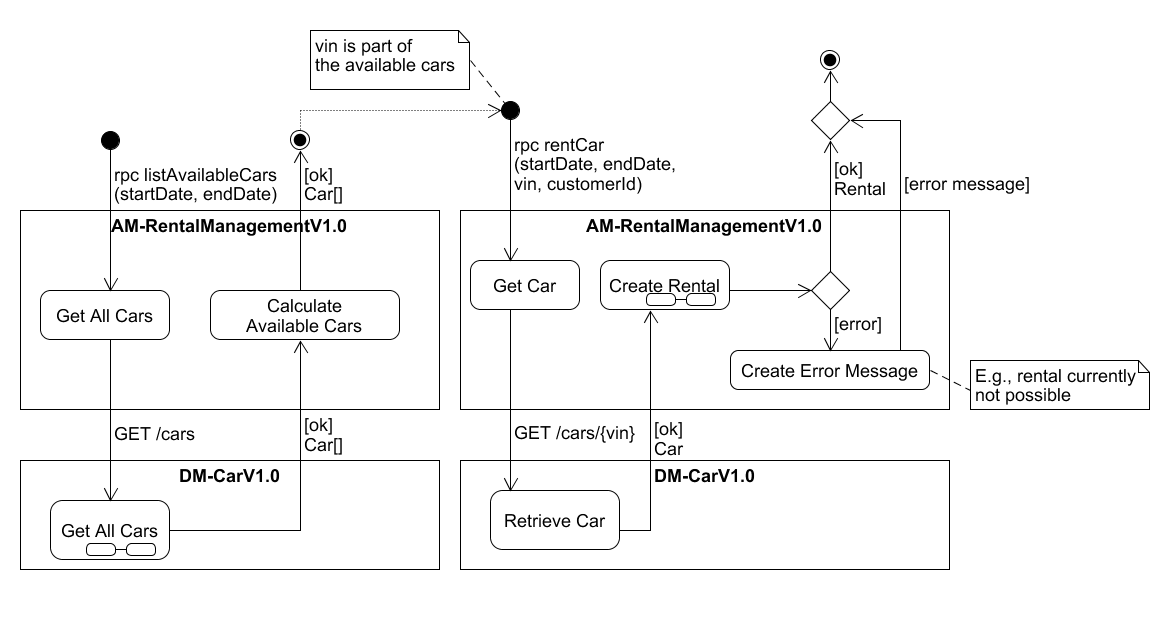
\includegraphics[width=0.8\textwidth]{figures/microservices/rentalManagement/ms_rentalManagement_orchestrationAddACar.png}
    \caption{Orchestration Diagram RentACarV1.0 (AM-RentalManagementV1.0)}
    \label{fig:ms_rentalManagement_orchestrationAddACar}
\end{figure}

\subsubsection*{Orchestration Between AM-Rentalmanagement and DM-Car}
% What triggers the orchestration diagram of "Rent a Car"
Two possibilities occur to trigger the orchestration diagram.
The first possibility is calling "\texttt{listAvailableCars}".
After the call is done, the second call is possible.
According to the specification of the orchestration diagram \cite{CM-G-ORC}, the gRPC call to \texttt{rentCar} is by the customer, who selects one of the listed cars to rent.
Therefore the call is triggered by the customer and therefore by the UI.

% Illustrate data flow between AM-RentalManagement and DM-Car in the orchestration
The data flow is as follows:
First, the RPC call is initiated to the application microservice.
The microservice then tries to get the requested car by calling the \texttt{GET} method on the \texttt{/cars/\{vin\}} path of the domain microservice.
After the domain microservice retrieves the car, it returns it to the application microservice which then creates the rental.
The termination of the function is decided whether creating the rental was successful or not. 
% What are possible responses from the orchestration diagram before termination
Here, two responses of the \texttt{rentCar} function are possible.
The responses are given by the AM and are modeled according to the outcome of \texttt{Create Rental}.
The first response is "\texttt{Create Error Message}".
It is triggered if an error during the creation of the rental occurs, for example, if the rental is currently not possible.
The operation then terminates prompting the error message.
The second response is a composite of the HTTP \texttt{OK} status code and the newly created rental. 
% How does UI-CarRental differentiate between the different responses
The UI therefore can differentiate between the responses by the given error.
